\section{Challenges}

\hidenum
\begin{frame}[noframenumbering]
\frametitle{Contents}
 \tableofcontents[currentsection,hideallsubsections]
\end{frame}
\shownum


\subsection{Challenges}

\begin{frame}
  \begin{block}{Challenges}
    \begin{itemize}[<+-|alert@+>]
      \item Perceptions.
      \item Library loading.
      \item Profiling.
    \end{itemize}
  \end{block}
\end{frame}


\begin{frame}
  \begin{block}{Covariance Revisited: Distributed Data Parameter Calibration}
    \begin{center}
     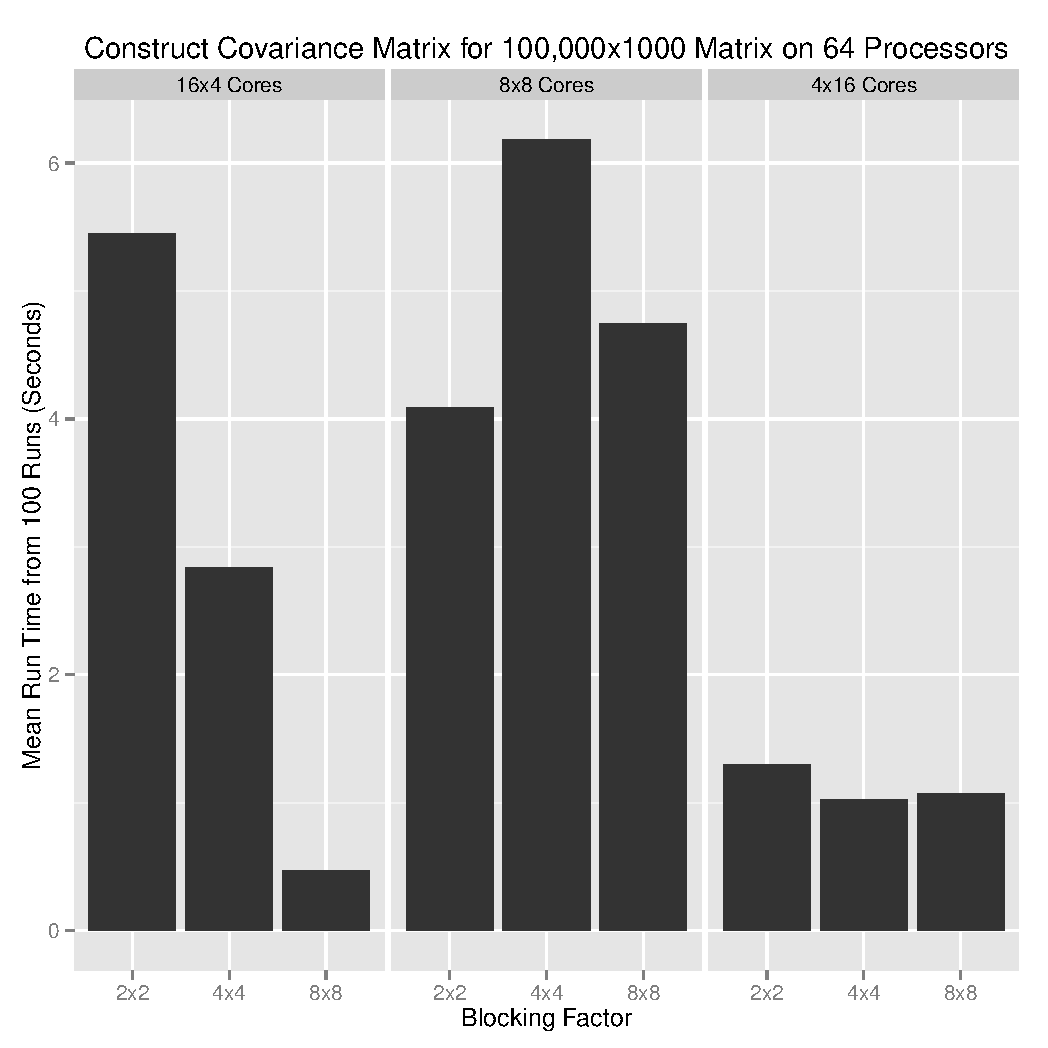
\includegraphics[width=10cm, height=7cm]{../common/pics/cov_param}
    \end{center}
  \end{block}
\end{frame}

\begin{frame}
  \begin{block}{Adding More Levels of Parallelism}
    \begin{center}
      {\color{dkblue}Distributed Memory (cluster nodes)} \\
      {\color{dkgreen}Shared Memory (multicore)} \\
      {\color{purple}Co-Processor (GPU, manycore)}
    \end{center}
    \begin{itemize}
      \item {\color{dkblue}pbdDMAT} + {\color{purple}CUBLAS}: near term on Titan 
      \item {\color{dkblue}pbdDMAT} - {\color{dkblue}ScaLAPACK} +
        {\color{dkblue}D}{\color{dkgreen}PLASMA}: QR only 
      \item {\color{dkblue}pbdDMAT} + {\color{dkgreen}PLASMA} or
        {\color{dkgreen}MKL} or {\color{dkgreen}ACML}: often helps 
      \item {\color{dkblue}pbdDMAT} + {\color{purple}MAGMA}: may not help 
    \end{itemize}
  \end{block}
\end{frame}

\begin{frame}
  \begin{block}{Tutorials}
  \begin{itemize}
    \item {\small OLCF Very Large Data Workshop
         ... {\color{red} NEXT!}}
    \item {\small Seoul National University, August 20}
    \item {\small SC13, November 17-22, Denver}
  \end{itemize}
  \end{block}
  \begin{block}{Invited Talks}
  \begin{itemize}
    \item {\small International Association for Statistical Computing, Aug 22-23, Seoul}
    \item {\small 59th ISI World Statistics Congress, August 25-30, Hong Kong }
  \end{itemize}
  \end{block}
\end{frame}

\hidenum
\section*{}  
\begin{frame}[noframenumbering]
 \begin{block}{Thanks for coming!}
 \begin{center}
     {\Large Questions?}\\[1cm]
     {\Large Be sure to stick around for the tutorial!}
  \end{center}
 \end{block}
\end{frame}
